%!TEX TS-program = xelatex

\documentclass[12pt]{article}
%%% This file is the preamble for the Pomona Linguistics LaTeX Paper Template, which is also used for the Quick Reference Guide. If you are brand new to writing with LaTeX, we suggest NOT messing with it, and just writing your paper using the Paper Template. If you are getting more comfortable in LaTeX and want to add packages and commands, this is where you do it (when using this template).

%For stacking text, used here in autosegmental diagrams
\usepackage{stackengine}

%To combine rows in tables
\usepackage{multirow}

%geometry helps manage margins, among other things.
\usepackage[margin=1in]{geometry}

%Gives some extra formatting options, e.g. underlining/strikeout
\usepackage{ulem}

%For putting links into papers, also helps make cross-references in the paper smart references
\usepackage[colorlinks = true,
            linkcolor = blue,
            urlcolor  = blue,
            citecolor = blue,
            anchorcolor = blue]{hyperref} %smarter cross-references, these options turn links blue

%Use package/command below to create a double-spaced document, if you want one. Uncomment BOTH the package and the command (\doublespacing) to create a doublespaced document, or leave them as is to have a single-spaced document.
%\usepackage{setspace}
%\doublespacing 

%paragraph formatting
\usepackage[parfill]{parskip}
\setlength{\parskip}{5pt} %plus 1 minus 1}
\setlength{\parindent}{30pt}
\usepackage{titlesec}

%use for special OT tableaux symbols like bomb and sad face. must be loaded early on because it doesn't play well with some other packages
\usepackage{fourier-orns}

%Basic math symbols 
\usepackage{pifont}
\usepackage{amssymb}

%%%Gives shortcuts for glossing. The use of this package is NOT explained in the Quick Reference Guide, but the documentation is on CTAN for those that are interested. MJKD finds it handy for glossing. (https://ctan.org/pkg/leipzig?lang=en)
\usepackage{leipzig}

%Tables
\usepackage{caption} %For table captions
\usepackage{booktabs} %helps format tables

%For citations and bibliography - as of 9.1.2019 we don't explain citations in this Quick Reference Guide, but Pedro Martin's tutorial does (see links in the Guide).
\usepackage{natbib}

%For OT-style tableaux
\usepackage{ot-tableau}

%Fonts
\usepackage[no-math]{fontspec} %This allows you to enter (via an IPA kayboard) IPA fonts and other symbols directly into LaTeX. Requires a particular setyp, see below.
\usepackage{libertine} %A font that actually contains many IPA symbols. This is the font you see in the preview to the right.

%to use these fonts, be sure that your typesetting engine is set to "XeLaTeX." In Overleaf, go to the Menu link on the top left (by the Overleaf icon), and under Settings be sure that the Compiler is set to "XeLaTeX." If you accessed this document via the Overleaf Pomona Linguistics template, all of this was already done for you.

%The Pomona Linguistics Paper Template in Overleaf is already set up for this, but you may run into this problem if you start building your own documents.

%highlights text with \hl{text}
\usepackage{color, soul}

%Drawing Syntax Trees
\usepackage[linguistics]{forest}

%This specifies some formatting for the forest trees to make them nicer to look at
\forestset{
  nice nodes/.style={
    for tree={
      inner sep=0pt,
      fit=band,
    },
  },
  default preamble=nice nodes,
}

%% For numbered and glossed examples %%
\usepackage{gb4e}



%Changes the \maketitle command to be smaller and take up less space on a page. 
\makeatletter         
\def\@maketitle{   % custom maketitle 
\noindent {\Large \bfseries \color{black} \@title}  \\ \hrule \noindent \@author \\ \@date  
}

%The code below will draw a circle around a piece of text. This is very useful for drawing attention to a word in a data example. use the command \circled{text} where the argument (`text' here) is what you want to be circled. This is illustrated in the Quick Reference Guide and the Paper Template.

\usepackage{tikz}

\newcommand{\circled}[1]{\begin{tikzpicture}[baseline=(word.base)]
\node[draw, rounded corners, text height=8pt, text depth=2pt, inner sep=2pt, outer sep=0pt, use as bounding box] (word) {#1};
\end{tikzpicture}
}


%%%%%%%%%%%%%%%%%%%%%%%%%%%%%%%%%%%%%%%%%%%%%%%%%%%%%%%%%%%%
%%%%%%%%%%%%%%%%%%%%%%%%%%%%%%%%%%%%%%%%%%%%%%%%%%%%%%%%%%%%

% Useful Ling Shortcuts

\RequirePackage{leipzig}
%\RequirePackage{mathtools} % for \mathrlap

% % % Shortcuts  (borrowed from JZ, I'm still unsure exactly what xspace requires)
\RequirePackage{xspace}
\xspaceaddexceptions{]\}}

%This makes the \emptyset command be a nicer one
\let\oldemptyset\emptyset
\let\emptyset\varnothing
\newcommand{\nothing}{$\emptyset$}

%Not all of these are explained in the Quick Reference Guide, but they are here bc they are relevant to some of our students.
\newcommand{\1}{\rlap{$'$}\xspace}
\newcommand{\0}{\rlap{\textsuperscript{$ˆ{\circ}$}}\xspace}
\newcommand{\Lb}[1]{$\text{[}_{\text{#1}}$ } %A more convenient left bracket
\newcommand{\Rb}[1]{$\text{]}_{\text{#1}}$ } %A more convenient left bracket
\newcommand{\gap}{\underline{\hspace{1.2em}}}
\newcommand{\vP}{\emph{v}P}
\newcommand{\lilv}{\emph{v}}
\newcommand{\Abar}{A$'$-} %A more convenient A-bar notation
\newcommand{\ph}{$\varphi$\xspace} %A more convenient phi
\newcommand{\pro}{\emph{pro}\xspace}
\newcommand{\subs}[1]{\textsubscript{#1}} %A more convenient subscript
%\newcommand{\hd}{$^{\circ}$\xspace} %Symbol for printing head / degree symbol
\newcommand{\spells}{$\Longleftrightarrow$} %spellout arrow for morph spellout rules
\newcommand{\tr}[1]{\textit{t}\textsubscript{\textit{#1}}} %easy traces with subscript
\newcommand{\supers}[1]{\textsuperscript{#1}}

% Abbreviations for glossing, based on Leipzig
\newleipzig{hab}{hab}{habitual}
\newleipzig{rem}{rem}{remote}
\newleipzig{sm}{sm}{subject marker}
\newleipzig{t}{t}{tense}
\newleipzig{aa}{aa}{anti-agreement}
\newleipzig{pron}{pron}{pronoun}
\newleipzig{rec}{rec}{recent}
\newleipzig{om}{om}{object marker}
%\newleipzig{ipfv}{ipfv}{imperfective}
\newleipzig{asp}{asp}{aspect}
\newleipzig{lk}{lk}{linker}
\newleipzig{pcl}{pcl}{particle}
\newleipzig{stat}{stat}{stative}
\newleipzig{ints}{ints}{intensive}
\newleipzig{ascl}{ascl}{assertive subject clitic}
\newleipzig{nascl}{nascl}{non-assertive subject clitic}
\newleipzig{ta}{ta}{tense and/or aspect}
\newleipzig{assoc}{assoc}{associative marker}
\newleipzig{hon}{hon}{honorific}
%\newleipzig{whprt}{wh}{\wh particle}
\newleipzig{sa}{sa}{subject agreement}
\newleipzig{conj}{conj}{conjunction}
%\newleipzig{loc}{loc}{locative}
\newleipzig{expl}{expl}{expletive}
\newleipzig{rcm}{rcm}{reciprocal marker}
\newleipzig{pers}{pers}{persistive}
%\newleipzig{}{}{} %this is just to copy for when I want to add more

%%%%%%%%%%%%%%%%%%%%%%%%%%%%%%%%%%%%%%%%%%%%%%%%%%%%%%%%%%%%
%%%%%%%%%%%%%%%%%%%%%%%%%%%%%%%%%%%%%%%%%%%%%%%%%%%%%%%%%%%%

%A couple of packages that seemed to prefer being called toward the end of the preamble

%This package provides macros for typesetting SPE-style phonological rules.
\usepackage{phonrule}

%For using Greek letters outside of math mode.
\usepackage{textgreek}


%Random, lets us use the XeLaTeX logo. Not important to the template at all.
\usepackage{metalogo}


%%%%%%%%%%%%
%% This is the end of the PREAMBLE
%%%%%%%%%%%



\title{Parallel implementation of zlib compression \& decompression}
\author{\textbf{Authors: Pengyun Zhao, Zian Ke}\\\textbf{Andrew ID: pengyunz, ziank}}

\date{\today}

\begin{document}


\maketitle
\section{Summary}
    We parallelized \href{https://www.zlib.net/}{zlib}, a library used for data compression and decompression, and achieved a \textbf{38$\times$} speedup on 36-core AWS machines compressing files of 1GB.
\section{Background}
    The key algorithms used by zlib to achieve data compression and decompression are the FLATE algorithms. The DEFLATE algorithm takes uncompressed data as input and produce compressed data as output. The INFLATE algorithm takes compressed data as input and produce uncompressed data as output. The FLATE algorithms are a combination of Huffman Coding and LZ77 compression, which will be explained briefly here.
    \subsection{Huffman Coding}
    Huffman Coding is a form of prefix coding that is commonly used for lossless data compression. The idea lies in that instead of using uniform number of bytes for all possible characters, we want to use smaller number of bytes to represent commonly used characters and do not mind using more bytes for less commonly used characters so that overall we are using fewer bytes to represent the characters.\\
    The process of Huffman Coding is basically constructing a single binary tree (``Huffman Tree'') and using the path to the element to represent to the element itself.\\
    In other words, do the following to an alphabet (set of all unique characters used), do the following till there is only one element in the set:
    \begin{enumerate}
        \item Take 2 elements with the lowest frequency.
        \item Join the two elements together, with the one with lower frequency being the '0' branch and the one with higher frequency being the '1' branch.
        \item Put the joined ``element'' back into the alphabet
    \end{enumerate}
    Then by the end, we will have a single binary tree where the paths to all the characters can be represented by 0s and 1s. We have shorter paths for characters with higher frequencies and (potentially) longer paths for characters with lower frequencies.\\
    An example would be 5 characters \{A, B, C, D, E\} with frequency \{0.10, 0.15, 0.30, 0.16, 0.29\}, then after using Huffman Coding the coding that represents the alphabets will be \{010, 011, 11, 00, 10\}, so instead of using ASCII codes which are 8 bits long we can use at most 3 bits to represent all characters.\\
    Of course, in order to decompress data we need to have the ``Huffman Tree'' constructed in order to translate the compressed characters back to their original form, and therefore the ``Huffman Tree'' is a \textbf{key data structure} used in the FLATE algorithms.
    \subsection{LZ77 Compression}
    LZ77 compression works by finding sequences of data that are repeated. It then replace repeated occurrences of data with references to a single copy of that data existing earlier in the uncompressed data stream and encodes a match by a pair of numbers known as the ``length-distance pair''. For example if we have the following string:\\
    \begin{center} Blah blah blah blah blah blah! \end{center}
    Then after using LZ77 compression it will become something like this:\\
    \begin{center} Blah b[Distance = 5, L=18]! \end{center}
    And it means that a same pattern has occurred before just 5 bytes ahead and we can repeat the pattern until we have reached 18 bytes, and this produces exactly the same string compared to the one before the compression, and saves a lot of bytes (of course in the actual implementations special characters and expressions are used to indicate a match instead of actual brackets because this may cause confusion with other characters that are originally in the uncompressed data).
    \subsection{Combining Together}
    The FLATE algorithms basically do the following:
    \begin{enumerate}
        \item Break input data stream into blocks.
        \item For each block, if we are now doing DEFLATE, apply LZ77 compression followed by Huffman Coding, store information about the constructed Huffman Tree. If we are doing INFLATE, apply the inverse of Huffman Coding first using the information stored in the compressed block, then apply the inverse of LZ77 compression to get the original uncompressed data.
        \item Output the processed blocks.Also there are 3 modes of compression available to the compressor and each block uses a single one of them to optimize compression efficiency.\\
    \end{enumerate}
    A simple explanation in figures would look like follows:
    \newpage
    \begin{figure}[!h]
    \begin{center}
    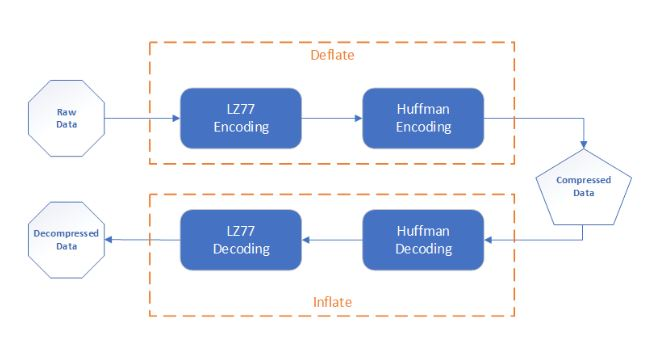
\includegraphics[height=7cm]{Diagram.JPG}
    \caption{The FLATE Algorithms Illustration}
    \end{center}
    \end{figure}
    \subsection{Identifying Workload Characteristics \& Dependence}
    The workload consists of the following parts:
    \begin{enumerate}
        \item Read from input (I/O intensive)
        \item Apply FLATE algorithms (Computationally expensive)
        \item Write to output (I/O intensive)
    \end{enumerate}
    We can see that the only key data structure used in the algorithm is the ``Huffman Tree'' and the key operation on it is to use paths to decode characters for compression, but it is not an ideal target for parallelism - it is bound with blocks of data, which is the smallest unit of computation in the algorithm (breaking it down further will also break down consistency).\\
    But when we look at the workload, we can see that the most (and only) computationally expensive parts are applying the FLATE algorithms to the input blocks to produce the output blocks, but this process is perfectly suited for parallelism, since the blocks are mostly independent from each other and every output block is computed from exactly one input block and does not depend on any other input blocks.\\
    One of the dependencies that currently exists is the block size. In the sequential version of the program, the length of a block is decided based on several factors, such as the size of the Huffman Tree, number of duplicates, etc. But in the parallel version it may cause a lot of extra communication. But a simple way to fix this would be to fix block sizes to eliminate the dependency, though with a little sacrifice of performance (but comes with a huge performance boost brought by parallelism, as will be analyzed in the results section).\\
    The greatest dependency in the program, of all, is that the output blocks need to be in the same order as the input blocks, but it is very simple to resolve since we can simply order the blocks computed in parallel fashion and compose the final output using the ordered blocks.\\
    Thus, zlib has a great potential for parallelism (nearly all the computationally extensive parts can be parallelized) and we can see that it is completely data-parallel because the blocks never have to talk to each other during the compression process, which is very like SIMD execution since we are just applying the same process to every block in parallel.
\section{Approach}
    Our implementation is based on parallel implementations \href{https://github.com/klauspost/pgzip}{pgzip} by Klaus Post and \href{https://zlib.net/pigz/}{pigz} by Mark Adler, one of the authors of zlib.\\
    After determining that the program is data parallel, we decided that partitioning the work of compression (decompression) and writing the processed blocks to output will be a good idea.
    \subsection{The Language We Chose and Why We Choose It}
    The language we chose is Go because it has many advantages compared to C/C++.\\
    In Go, a thread is called as a \textbf{goroutine} and it is quite different from C/C++ threads, it has several great advantages which are the reasons we chose Go to implement the program:
    \begin{enumerate}
    \item \textbf{Managed by Go runtime.} Goroutines are managed by Go runtime and has no hardware dependencies and thus adapts to different platforms better.
    \item \textbf{Low-latency communication between threads and natural synchronization.} This is the \textbf{most important reason} we chose Go. Goroutine uses \href{https://tour.golang.org/concurrency/2}{channels} to communicate with each other, the channels have a very low latency of communication that is very similar to MPI Send and Recv, but much easier to use and express (built-in support from Go).\\
    Also, channels preserve the order of sending and receiving, so they can also be used to guarantee the order of messages (also they block on receive when nothing has been sent and for buffered channels whose sizes are specified they block on send when the channels are filled with message that haven't been received) and thus act as natural synchronization primitives.
    \item \textbf{Little overhead for setup and teardown.} goroutines are created and destroyed by the Go runtime. These operations are very cheap compared to threads as go runtime already maintain pool of threads for goroutines. In this case OS is not aware of goroutines, so we \textbf{save one level of abstraction}.\\
    Also this allows us to be more generous on spawning goroutines and thus enables program design to be simpler. This is very similar to the comparison between ISPC gangs and pthreads talked about in the first few lectures.
    \item \textbf{Low scheduling cost.} goroutines are cooperatively scheduled so fewer values need to be saved or restored when switching goroutines.
    \end{enumerate}
    So we can see that go combines advantages from several programming languages or frameworks we have seen in class and thus we evaluated go to be a better choice to achieve higher performance boost.\\
    Our target machines are machines with large number of processors (that also means more caches at the same time), enough memory to process multiple blocks in memory, some examples of these machines will be GHC machines and AWS machines (we will be using c5.9xlarge in this project).
    \subsection{A Detailed Explanation of the Parallelism Scheme}
    Compared to the sequential version the following new data structures are added to ensure concurrency and consistency:
    \begin{itemize}
        \item A job queue to record the order of blocks. This is implemented via a buffered channel with a size due to the characteristics of channel described above. The size of the job queue is set to be the number of processors set via a function provided in our implemented of the library (by default it is set to the number of processors on the machine), so it achieves some degree of \textbf{load balancing}, somewhat similar to OpenMP's dynamic scheduling, but with much less overhead.
        \item For each block, we will allocate a unique data structure for it to store processed block \textbf{for that single block}, this is more like a pointer to completed partition in C/C++, but with much lower latency and storage overhead. This also implemented using channels, but different from the shared job queue it is unique for every single block.
    \end{itemize}
    The mapping of the work is as follows (illustrated via a figure first):
    \begin{figure}[!h]
    \begin{center}
    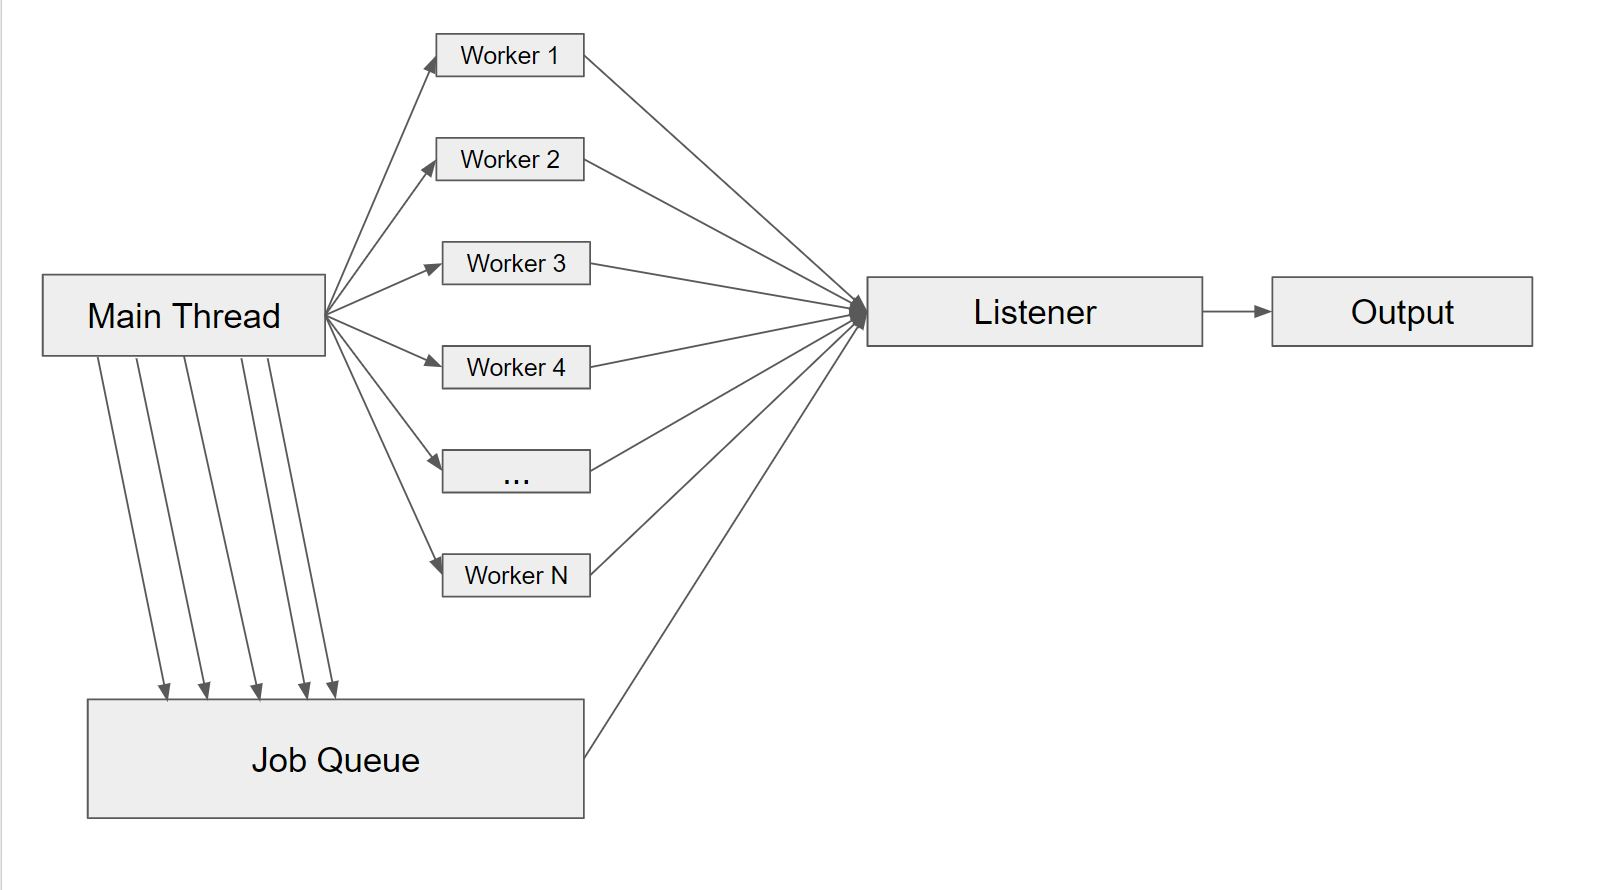
\includegraphics[height=7cm]{Procedure.JPG}
    \caption{How Parallelism is Achieved}
    \end{center}
    \end{figure}
    ~\\
    The detailed procedure is as follows:
    \begin{enumerate}
        \item The main thread breaks data into blocks using the specified block size. Note that this feature is not present in the sequential versions of zlib taking official go implementations as an example because in the sequential version data is continuous so the block size can vary based on current state of the data such as how many duplicates are there and the size of the Huffman tree, etc. In the parallel version we want to eliminate data dependency as much as possible so each block size (in terms of raw data) is fixed.
        \item The main thread first starts a new goroutine that acts as the listener to monitor worker threads.
        \item The main thread then for each block puts a reference (more precisely a channel) to the block into the job queue in order and starts a new goroutine worker thread for the block with a FLATE compressor initialized.
        \item Each work thread works on compressing (decompressing) the data independently and sends a notification via the unique channel bound to the block when the work is done. The job queue is a buffered channel so at most \texttt{NUM\_PROCESSOR} worker threads can be working on it at the same time. When a work thread returns, a new worker thread unblocks and can start working (load balancing using the channel). This enables a better mapping of threads to cores.
        \item The listener thread takes the reference out from the job queue one by one (resolving order dependency), it blocks until it has received notification from the worker thread responsible for that block sent via the reference that work has completed, then the listener receives compressed (decompressed) data from the worker thread and writes it to output (the worker thread exits after sending the notification and data via the channel).
        \item The main thread blocks until all the blocks have been processed and written. Then the main thread (the writer in user's eyes) closes the job queue (at this time the listener returns when it detects the job queue is closed) and can be closed, flushed or reset.
    \end{enumerate}
\section{Results}
    \subsection{Performance and Experiment Setup}
    We benchmarked our program on an \textbf{AWS c5.9xlarge machine with 36vCPUs, 72GiB RAM and an EBS Bandwidth of 4.5Gbps}, using the built-in test function supported by go:\\
    \begin{center} go test pzlib-benchmark -v -count=1 -bench=. -benchtime=10s\end{center}
    where the run option specifies the tests to run, the count option enforces no cached tests, the benchmark option specifies the benchmarks to run (different from test where tests are used to check the correctness of the implementation), and the benchtime option makes sure that we have enough time to run the benchmarks for enough number of iterations before go shuts down the benchmark by force. The benchmark option will output the average running time it takes to finish a task, which is what we used to measure our program's performance.\\
    There are 2 types of benchmarks we have conducted:
    \begin{enumerate}
        \item We measured the running time of our parallel zlib implementation against the official sequential implementation and for some conditions (problem sizes) we also used it to draw a speedup graph with respect to different number of cores under different values of the condition.
        \item We also measured the running time for 4 different zlib programs:
        \begin{itemize}
            \item The official zlib implementation.
            \item An improved sequential \href{https://github.com/klauspost/compress/tree/master/zlib}{zlib implementation} by Klaus Post, the author of pgzip.
            \item pzlib-std, one of our intermediate implementations that used the official ``compress/flate'' library and unsafe functions to reset the dictionary.
            \item pzlib, our final implementation that uses the improved ``\href{https://github.com/klauspost/compress/tree/master/flate}{compress/flate}'' by Klaus Post.
        \end{itemize}
        We then compared and analyzed the running time of those 4 implementations.
    \end{enumerate}
    We set up the experiments by first analyzing the general performance of our implementation, which is accomplished by feeding files to the 4 different zlib implementations and measuring the time they take to finish the whole compression (from start of compression to the end of compression) and then comparing the time against each other. Then specifically for our final parallel implementation of zlib, we generated different files representing different workload characteristics and measured the time it take to compress those files under different conditions against the time it took for the official implementation.\\
    We benchmarked our program considering the following factors (i.e. these are our problem sizes):
    \begin{itemize}
        \item \textbf{Different file sizes.} How well does our implementation perform on different file sizes?
        \item \textbf{Different block sizes.} How well does our implementation perform on different block sizes?
        \item \textbf{Different compression levels.} How well does our implementation perform on different compression levels (1-9)?
        \item \textbf{Different file characteristics.} How well does our implementation perform on files that have different characteristics? Files whose contents are completely duplicate? Files whose contents are purely random?
    \end{itemize}
    Also a paragraph on using AWS as required for using AWS credits:\\
    Using AWS grants us a lot more resources (CPU, memory) compared to GHC machines, which allows us to benchmark our implementations on more processors and extend our analysis further. Also using AWS gives us more freedom to install and use different programs and frameworks, which can be very helpful sometimes.
    \subsection{General Results}
    We first measured the running time of the 4 implementations compressing a JSON file of 1GB using the Country Travel Information dataset found at \href{https://catalog.data.gov/dataset/country-travel-information}{the US Government's Open Data Website}, and here are the results (normalized using pzlib's running time as reference):
    \newpage
    \begin{figure}[!h]
    \begin{center}
    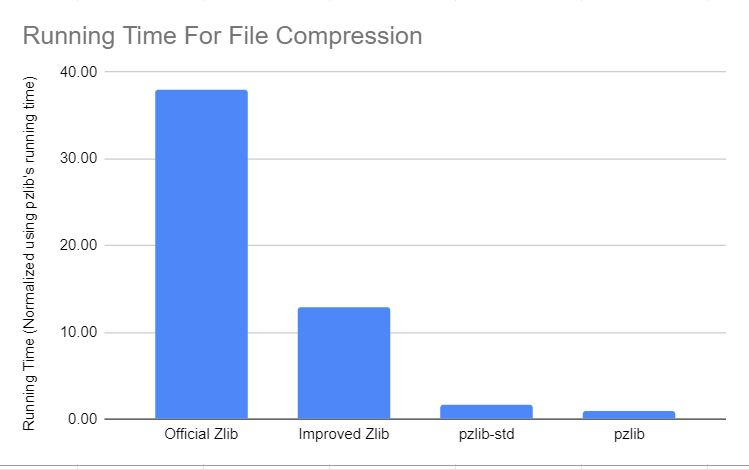
\includegraphics[height=6cm]{GeneralResults.JPG}
    \caption{General Running Time of the 4 Implementations}
    \end{center}
    \end{figure}
    ~\\
    Here we can see that pzlib achieves a great speedup compared to zlib, with a speedup of 38x on a 36-core machine, which is linear (or even superlinear), this proves our analysis in the background section that zlib is data-parallel, meaning there is little dependence between data, thus enabling our parallelized version to have a high arithmetic intensity and achieve linear (superlinear) speedup.\\
    We can also see that compared to ``compress/zlib'', which is an improved version implemented by Klaus Post, the author of pgzip, we are only able to achieve a 12x speedup. The improved zlib sequential implementation used a modified FLATE package that is optimized for sequential FLATE algorithms, but it is not compatible with the parallelized version since in parallelized version we fix the length of the blocks in order to erase data dependency and this will hurt the performance of FLATE algorithms because in fixed size blocks Huffman Coding may not be able to produce an efficient Huffman tree and LZ77 compression may not be able to find duplicates, which is one of the sacrifices we mentioned in section 2 and 3.\\
    Compared to pzlib-std, our intermediate implementation, pzlib also performed better with a 1.8x speedup, with the only difference of pzlib-std using the official FLATE package from go and using an unsafe function to reset the dictionary, which again shows the importance of using an optimized FLATE package to adopt to the situation.\\
    Decompression tests show similar results, so in order to achieve further speedup, we may need to come up with a new implementation or optimization for the FLATE package.
    \subsection{Different File Sizes}
    We then want to know the affect of file sizes on the performance of pzlib, i.e. will pzlib behave differently on small files and larges.\\
    So we measured pzlib's running time of different number of cores (1,2,4,8,16,32) for files of different sizes (1KB, 10KB, 100KB, 1MB, 10MB, 100MB, 1GB) and plot the speedup against the corresponding running time of the sequential zlib, which is as follows:
    \newpage
    \begin{figure}[!h]
    \begin{center}
    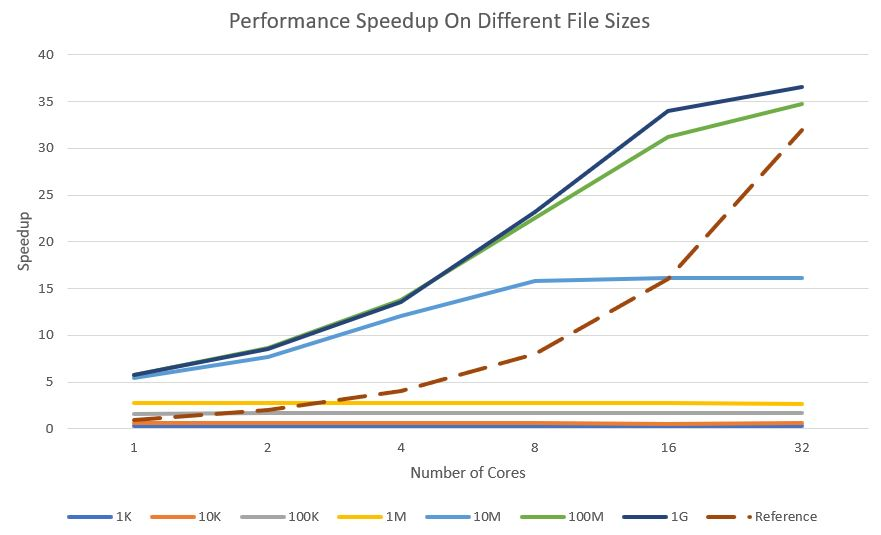
\includegraphics[height=8cm]{SpeedupFilesizes.JPG}
    \caption{Speedup On Different File Sizes}
    \end{center}
    \end{figure}
    ~\\
    There are mainly three interesting observations from this graph besides the one that the program achieves superlinear speedup when the file size is very large (100M and 1G):
    \begin{enumerate}
        \item When file sizes are very small, the speedup is constant and even a lot worse than the sequential version.
        \item When file sizes are larger but still smaller than the single block size (1M), the speedup is still constant, but a little bit better than the sequential version.
        \item When file sizes are larger than the single block size but not too much, the performance is superlinear but plateaus after some number of cores.
    \end{enumerate}
    The plausible reasons for these observations are:
    \begin{enumerate}
        \item When the file size is smaller than the single block size, we can of course only get one block to process, and this makes the parllelized version no different than the sequential version.
        \item Also since the block size is fixed in the parallel version, when the file size is too small, there are a lot of ``wasted spaces'' (filled with padding) that makes the FLATE algorithm for the parallelized version extremely inefficient (we are wasting our time on bytes that are not used).
        \item When file sizes are larger but still smaller than the single block size, we still only have one block and are essentially doing sequential work, but the utilization of the block is higher so the parallelized version starts to perform better than the sequential version.
        \item When file sizes are larger than the single block size but not too much, we have a number of blocks but it is smaller than the number of processors we have (36 vCPUs). So when the number of cores go past a threshold, some of the cores have no work to do and it is as if they don't exist.
        \item Also, when the file size increases, the percentage of overhead (block starts and ends, thread start overheads and context switch overheads for goroutines, etc.) has a less percentage in the total running time, thus increasing performance. (100M and 1G would be a good example, files of 1G seem to have a better performance than 10M and 100M at multi-core scenarios, even though they are all superlinear).
    \end{enumerate}
    \subsection{Different Block Sizes}
    Block size is also an important factor for the performance of pzlib and we also want to know the effect of it, namely how does pzlib perform on small and large block sizes?\\
    We then measure pzlib's performance speedup on different number of cores for different block sizes ranging from 16KB to 16MB, and here is the graph describing the speedup against the corresponding running time of the sequential version of zlib for a file of 100MB, which is as follows (the default block size is 1MB):
    \begin{figure}[!h]
    \begin{center}
    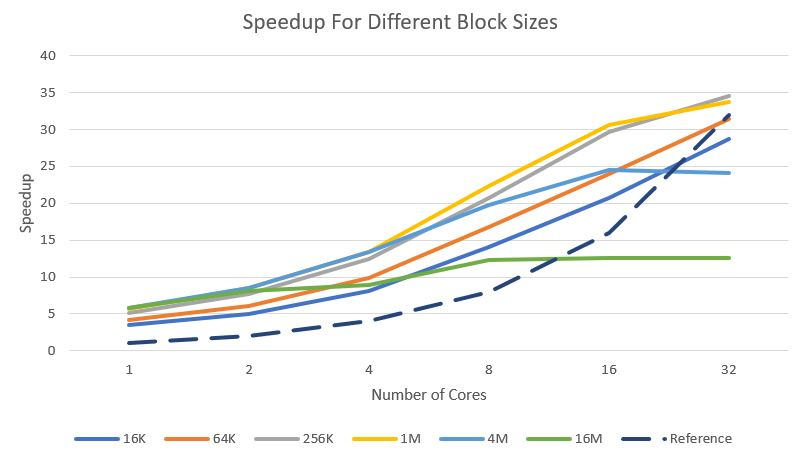
\includegraphics[height=8cm]{SpeedupBlocksizes.JPG}
    \caption{Speedup On Different Block Sizes}
    \end{center}
    \end{figure}
    ~\\
    Here we can see that pzlib performs best on moderate block sizes (256K-1M), and performs worse on either block sizes too small or block sizes too big (when block sizes are 4M and 16M the performance even go down with the increase in the number of cores used).\\
    Some plausible reasons for this behavior include:
    \begin{enumerate}
        \item When the block size is too small, there are a huge number of blocks as well as goroutines (according to the implementation described in the Approach section one goroutine and a separate channel will be created for each block). This increases the amount of communication and context switch as well as synchronization happening. Also since each block has to create a block start and block end, the amount of overhead greatly increases.
        \item When the block size is too large, even though the amount of overhead will decrease and the efficiency of the FLATE algorithms may increase, the number of blocks will become too small (sometimes smaller than the number of processors available), so there will be a lack of parallelism which will lower the speedup. Also, remember that each processor's L1 cache has limited space available, so when the block size is close to or greater than the processor's cache size (or even greater than the shared L2 cache's size) , we will repeatedly evict from cache and read from memory, which is memory inefficient.
    \end{enumerate}
    Therefore, our implementation works best on block sizes between 256K and 1M.
    \subsection{Different Compression Levels}
    We would also like to know our implementation's performance on different levels of compression, and want to compare two things:
    \begin{itemize}
        \item For the same file, how does compression level affect the running time.
        \item For the same file, how does the size overhead change between different compression levels.
    \end{itemize}
    So we benchmarked pzlib's performance on different compression levels from 1 to 9 on all processors possible (36 cores) and plotted 2 graphs describing the running time and the size overhead (default level is 6):
    \begin{figure}[!h]
    \begin{center}
    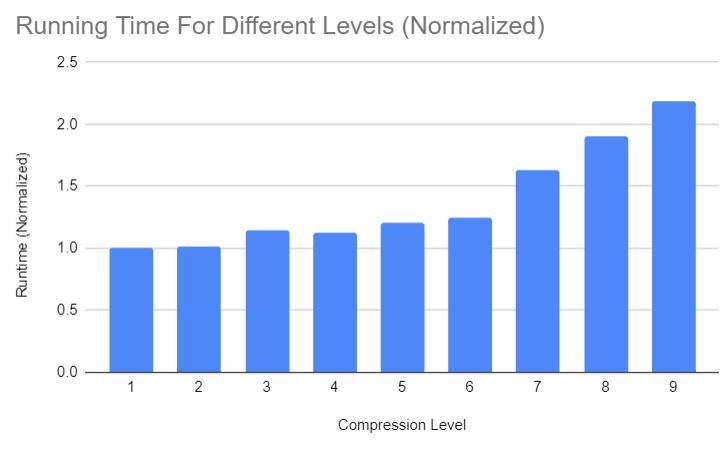
\includegraphics[height=8cm]{RuntimeCompressionLevel.JPG}
    \caption{Runtime for Different Compression Levels (Normalized)}
    \end{center}
    \end{figure}
    ~\\
    We can see that the running time increases when the level of compression level increases (especially for level 7,8,9), which is normal behavior since the amount of work we need to do increases.\\
    We then present a graph describing the change in size between uncompressed and compressed for different compression levels:
    \newpage
    \begin{figure}[!h]
    \begin{center}
    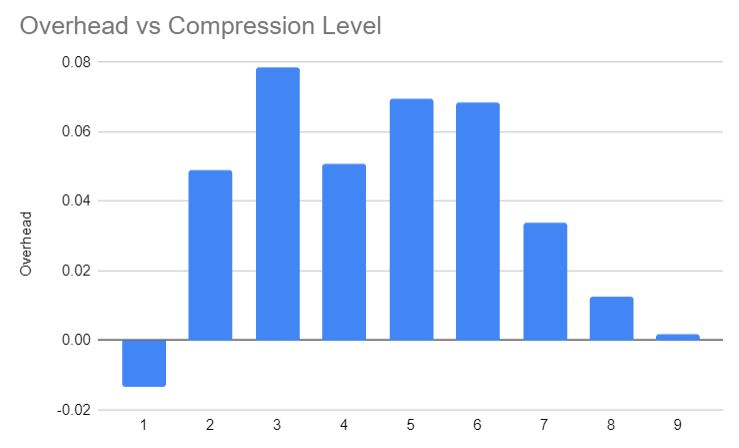
\includegraphics[height=8cm]{SizeOverheadCompressionLevel.JPG}
    \caption{Size Overhead Compared to zlib for Different Compression Levels (Relative)}
    \end{center}
    \end{figure}
    ~\\
    We can see that despite level 1 being an outlier, the size overhead of the results produced by pzlib compared to that of zlib, peaks at level 3 with a value of 8\%  and gradually decreases when the compression level increases. A plausible cause (this is a speculated guess) for the decreasing trend is that when the compression level is low, the required window size will be much smaller than the block size, which is 1MB, and when the compression level goes up, the required window size will also increase and 1MB will become a good fit for block processing.
    \subsection{Different File Characteristics}
    The final factor we want to research on is file content characteristics, based on how the FLATE algorithm works, will our current implementation has a great performance difference between files with all duplicates, all randoms, somewhere in between (in this project we are using the Json dataset mentioned previously to represent Json files and the full script of Hamlet to represent text files).
    We then benchmarked our implementation using the two mentioned above together with a file filled with `A's, and a file with totally random contents,  and measured the differences of running time and size overhead of compressed files:
    \newpage
    \begin{figure}[!h]
    \begin{center}
    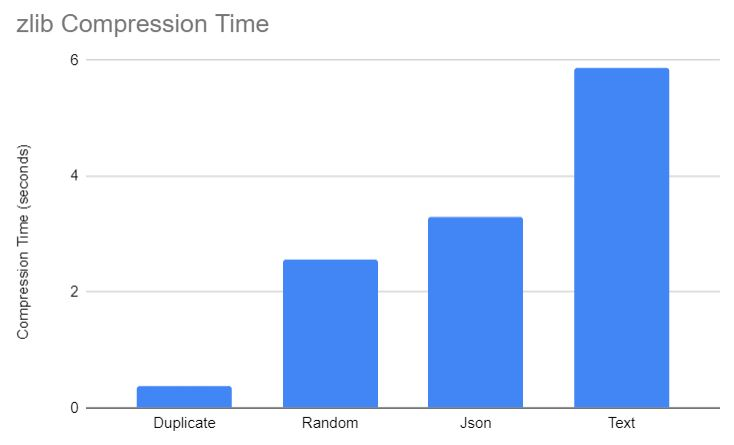
\includegraphics[height=8cm]{ZlibCompressionTimeFileChars.JPG}
    \caption{Running Time of zlib for Files with Different Characteristics}
    \end{center}
    \end{figure}
    ~\\
    \begin{figure}[!h]
    \begin{center}
    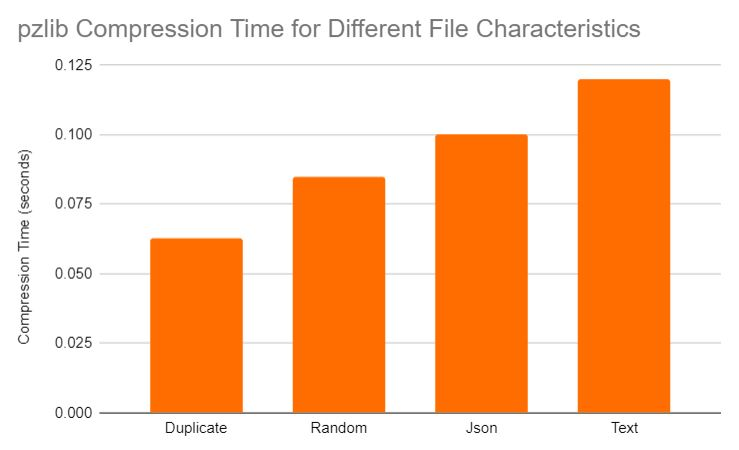
\includegraphics[height=8cm]{PZlibCompressionTimeFileChars.JPG}
    \caption{Running Time of pzlib for Files with Different Characteristics}
    \end{center}
    \end{figure}
    ~\\
    We can see that both zlib and pzlib has the fastest running time on completely duplicate content, followed by Json and then text, which shows that completely duplicate random and pure random allows the FLATE algorithm to run faster since in one of the cases the sliding window keeps growing while in the other case the sliding window has length zero most of the time. It shows that it is the cost of ending a sliding window of a moderate length that is the biggest (this is often the case in Json and text files).
    We then measured the size overhead of pzlib compared to zlib for the 4 different types of file characteristics and first compare them against each other for both zlib and pzlib:
    \begin{figure}[!h]
    \begin{center}
    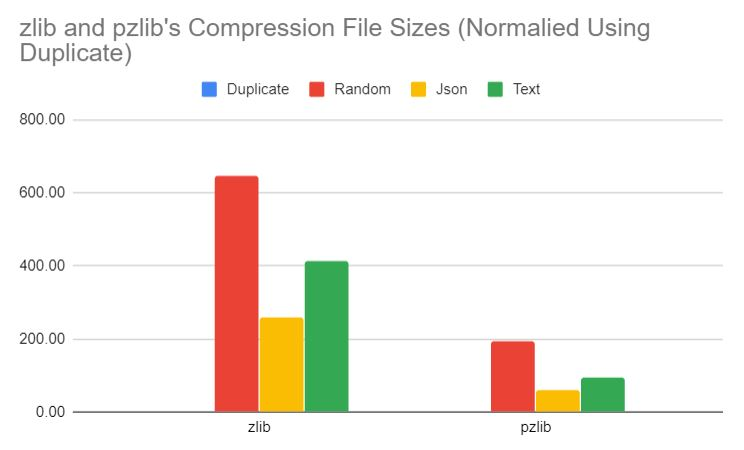
\includegraphics[height=8cm]{CompressionSizeFileChars1.JPG}
    \caption{Running Time of zlib and pzlib for Files with Different Characteristics (Grouped by program)}
    \end{center}
    \end{figure}
    ~\\
    Here we can see for both zlib and pzlib the sizes of the compression results are the smallest for file with all duplicates, followed by the ones for Json files, then text files and finally files with purely random content. And it is also the order of number of duplicates in file content: file with pure duplicate has of course the most duplicates, then Json (a lot of the fields are identical), followed by text and finally the purely random file.
    It is an apparent result according to the FLATE algorithm, but notice the size ratio of zlib is higher than the one for pzlib.\\
    A plausible reason for this is that in sequential zlib all duplicates are eliminated and replaced since block sizes are variable, but in pzlib it is possible that the stream of duplicates are cut due to fixed block sizes, causing the compressed file size to be much larger than the sequential case, we will see a much more precise demonstration and explanation of it in the figure below.\\
    We then group by different file characteristics and compare the compressed file sizes of zlib and pzlib for the same file:
    \newpage
    \begin{figure}[!h]
    \begin{center}
    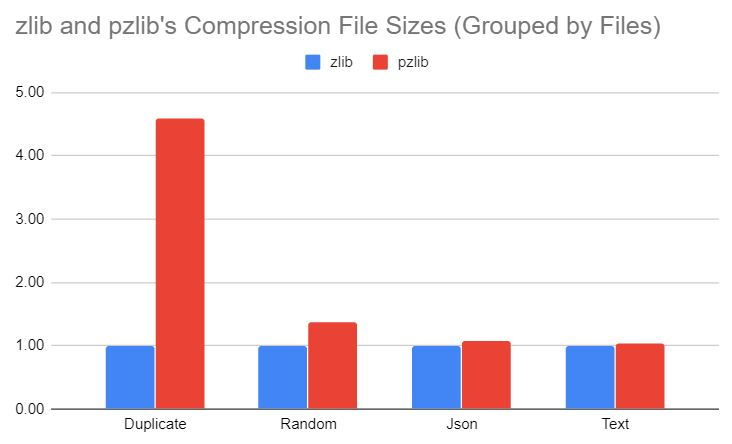
\includegraphics[height=8cm]{CompressionSizeFileChars2.JPG}
    \caption{Running Time of zlib and pzlib for Different Files (Grouped by files and normalized)}
    \end{center}
    \end{figure}
    ~\\
    Much worse then the measurement in the previous section, we find the size overhead under random scenarios to be 40\% and the one under all-duplicate scenarios to be 360\%, which is terrible. The obvious reason for this problem (again) is that we are using fixed-size blocks. Since in the sequential implementation the block size is variable, the ``sliding window'' can keep going and reducing duplicates as long as it keeps encountering duplicates. For example, a string of 10000 `A's in the sequential version can be reduced to something like `A'[D=1,L=9999]. However, this is not the case in pzlib, it is very possible that the sliding window will be ``cut in halves'', causing bytes that could've been compressed to be in a new block and thus not able to compressed into the previous block, so it may be something like A[D=1, L=999] repeated 10 times, which takes 10 times more space compared to the output of the sequential version, resulting in the overhead being more than 3 times the size of zlib's output for the all-duplicates case and 40\% overhead for the random case because for random contents you may potentially lose all chances of eliminating duplicates because of the problem mentioned above and this is especially painful for random contents since there may originally be very few duplicates.\\
    Therefore, considering both time and space efficiency pzlib is best to be run on files with moderate number of duplicates (meaning it has some kind of ``rules''). It does run faster on all-duplicate files, but comes with a huge price of space inefficiency.
    \subsection{Conclusion: Do we achieve our goals?}
    Based on the analysis from previous sections, our implementation works best on large files (larger than 100M) with a block size of around 256K-1M, with not too many duplicates. Our parallel implementation achieves significant speedup compared to sequential zlib. The biggest disadvantage of our implementation is that it usually has some size overhead compared to the sequential zlib and the problem essentially becomes a tradeoff between space and time.
    Some factors that could limit our speedup include:
    \begin{enumerate}
        \item \textbf{Files that are too small.} Small files will cause lack of parallelism and also increase processing overheads. And benchmarking shows that our implementation works best on files large enough (100M-1G seems to be a good fit, if files are too large then it will be hard for them to fit in memory completely).
        \item \textbf{Block sizes that are too small or too big.} Block sizes that are too small will increase both memory overheads (block starts and ends, additional data structures) as well as synchronization and communication overheads (more goroutines, thus more context switches and startup costs as well as communication between threads). Block sizes that are too big will cause lack of parallelism as well as memory inefficiency due to cache limitations.
        \item \textbf{The approach of our algorithm.} Our implementation of the parallelism approach directly divides data into fix-sized blocks. While this helps eliminate dependency between data and allows us to have superlinear speedups, it hurts the performance of the FLATE algorithm, both in terms of time (for a single core) and space. The most obvious problem is that using fix-sized blocks will introduce a very large size overhead (around 40\% normally and 360\% in the worst case) because the data dependency (such as the ``sliding window'' in LZ77 compression) in the sequential version that produces results with optimized space will often be ``cut in halves''. Therefore, we may need to research on new improvements or modifications to the FLATE package to try to preserve this depency as much as possible.
    \end{enumerate}
    Also we think we have a good choice of machine. Even though GPUs have much more cores than CPU,it has a limited size of shared memory (less than 64KB) which makes it not a good choice for zlib since the block size that has the performance will be around 256KB - 1MB.\\
    \textbf{To conclude}, we have pretty much realized all the deliverables we plan to have that are described in the project proposal and checkpoint:
    \begin{itemize}
        \item Implement a parallelized version of zlib in Go that produces correct compression and decompression results and is fully compatible with the standard Go zlib package (completed).
        \item Achieve noticeable speedup compared to the original sequential implementation (completed, we have 38x speedup on a 36-core machine).
        \item Have a comprehensive analysis on the implementation for different kinds of workloads (completed).
    \end{itemize}
    And as for the ``nice to haves'', we have achieved similar performance with the currently released versions of parallel implementations (faster than pigz and close to pgzip). We have also publicly released our source code as a Go package, as shown in the link below. But as for the other nice to haves (performance analysis on different machines, proof of efficiency) time is still needed, and the analysis we give in this report will provide valuable references for future development and improvement of pzlib.
\section{Project Code Link}
    The source code of the project is located at \href{https://github.com/zianke/pzlib}{https://github.com/zianke/pzlib}, while the benchmark files and project reports are located at \href{https://github.com/zianke/15618-final-project}{https://github.com/zianke/15618-final-project} (simply because they are too large to be put in the same repo with the source code).
\section{References}
\begin{itemize}
\item \href{https://github.com/klauspost/pgzip/blob/master/gzip.go}{pgzip by Klaus Post}
\item \href{https://github.com/golang/go/tree/master/src/compress/zlib}{The official implementation of zlib by Go}
\item \href{https://github.com/klauspost/compress/tree/master/zlib}{An improved version of zlib by Klaus Post}
\item \href{https://zlib.net/pigz/}{pigz, a parallel implementation of zlib in c by Mark Adler}
\item ``An Explanation of the Deflate Algorithm'', by Antaeus Feldspar
\end{itemize}
\section{Division of Work}
Equal work was performed by both project members, with Zian Ke being responsible for developing the program based on the references as well as implementing the test cases and Pengyun Zhao being responsible for designing the test cases and benchmark metrics, conducting benchmarks and analyze the measurements as well as writing the final report.
\end{document}
